% !! indica que tem que ser arrumado

O projeto aqui apresentando trata da inserção de funcionalidades em um sistema no qual o aluno Rodrigo Longhi Guimarães, sobre orientação dos professores André Schneider de Oliveira e João Fabro, já vem trabalhando desde meados de junho de 2014. Por se tratar de um projeto com vários termos técnicos foi feito um sumário que encontra-se no Apêndice. Esse projeto de iniciação científica consiste na preparação do robô Pioneer 3-AT para aplicação de um \textit{framework} de inteligência artificial baseado em agentes LIDA \cite{LIDA}. A preparação feita antes do início do atual trabalho consistiu em:

\begin{compactitem}
\item Desenvolvimento de uma estrutura em alumínio, capaz de suportar o \textit{netbook}, \textit{master} do ROS (\textit{Robot Operating System}), e eventuais sensores, como o Kinect.
\item Instalação do \textit{framework} ROS no \textit{netbook} e em outra máquina, além do estabelecimento da comunicação entre elas.
\item Instalação dos \textit{drivers} do Kinect no \textit{netbook}, de forma a enviar dados inteligíveis do sensor Kinect ao ROS.
\item Criação de uma placa, versão protótipo para o Arduino, que não suportava interrupções e lia todos os sensores por \textit{polling}.
\item Estabelecimento da comunicação da placa do Arduino com o ROS, na distribuição \textbf{Fuerte} ~\cite{rosFuerte} do ROS.
\item Iniciação dos estudos sobre navegação autônoma. Uma versão inicial da navegação foi desenvolvida, mas não se tinha muito conhecimento sobre seu funcionamento e a navegação era bastante problemática. O sistema de localização, \verb|gmapping|, não era funcional.
\item Desenvolvimento e adaptação de alguns pacotes não relacionados com o presente projeto, como pacotes de reconhecimento de voz, sintetização de fala, reconhecimento de pessoas, seguidor de pessoas, entre outros.
\end{compactitem}

Além do objetivo principal, que é a adaptação do robô para trabalhar com o LIDA, este projeto de iniciação científica acabou se desviando e o trabalho se deu com algumas tarefas que possibilitaram a participação do robô Pioneer 3-AT como competidor na categoria @Home da CBR2014, na qual o robô ficou em 3º lugar da América Latina ~\cite{cbr2014}. 

Vendo o grande potencial do projeto resolveu-se aprimorar a plataforma, com o objetivo de arrumar erros de funcionalidades já presentes e adicionar novas funcionalidades ao robô, tornando-o ainda mais competitivo no cenário da robótica doméstica. É isto que este atual trabalho de oficina de integração fez: melhorou a navegação autônoma, refez a parte de sensoriamento com o arduino e criou uma visualização 3D usando o pacote \verb|octomap|.

%A figura \ref{fig:visaoGeral} apresenta a visão geral do projeto. Este projeto foi desenvolvido com dois cenários reais em mente. O primeiro, figura (a), mostra um cenário em que o mapeamento tridimensional de um ambiente por um robô guiado por algum controle remoto (Wiimote) seja necessário. O segundo cenário, figura (b), mostra os sensores, o encoder e o Kinect atuando para gerar uma navegação autônoma (\textit{Simultaneous localization and mapping}) competente (ver requisitos funcionais para o que chamamos de competente..!!). 
%RODRIGO: MUDEI ESSE PARÁGRAFO AQUI, VEJAM SE ACHAM MELHOR:

A versão do ROS utilizada atualmente no projeto é a \textbf{Hydro} ~\cite{rosHydro}. Esta versão, por mais que não seja a mais atual, foi escolhida por suportar todos os pacotes que utilizamos e também pela sua maturidade.

O projeto atual foi desenvolvido com dois objetivos principais em mente: tornar um robô móvel capaz de realizar navegação autônoma e teleoperar este mesmo robô enquanto cria-se uma visualização 3D do ambiente. Na Figura \ref{fig:visaoGeral0}, é possível visualizar um diagrama que deixa evidente as comunicações do sistema, que são compostos por: dois computadores executando o \textit{framework} ROS e trocando mensagens entre si, além de um controle Wiimote que manda mensagens por \textit{bluetooth} aos computadores. Adicionalmente, na Figura \ref{fig:visaoGeral1}, são apresentados todos os sensores acoplados ao sistema, além do \textit{netbook}, que funciona como núcleo do ROS e gerencia todo o sistema.

\begin{figure}[H]
\centering
  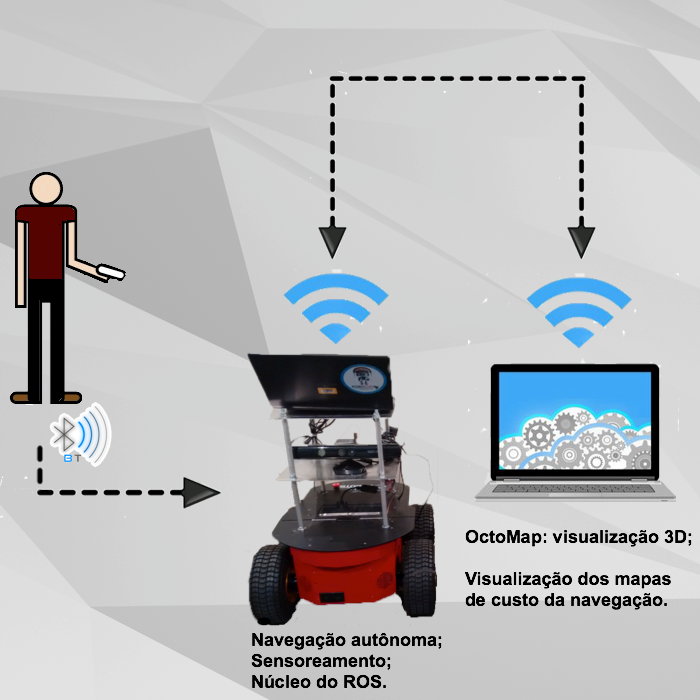
\includegraphics[width=8cm]{images/visaoGeral0.png}
\caption{\small{Visão geral da comunicação no sistema.}}
\label{fig:visaoGeral0}
\end{figure} 

\begin{figure}[H]
\centering
  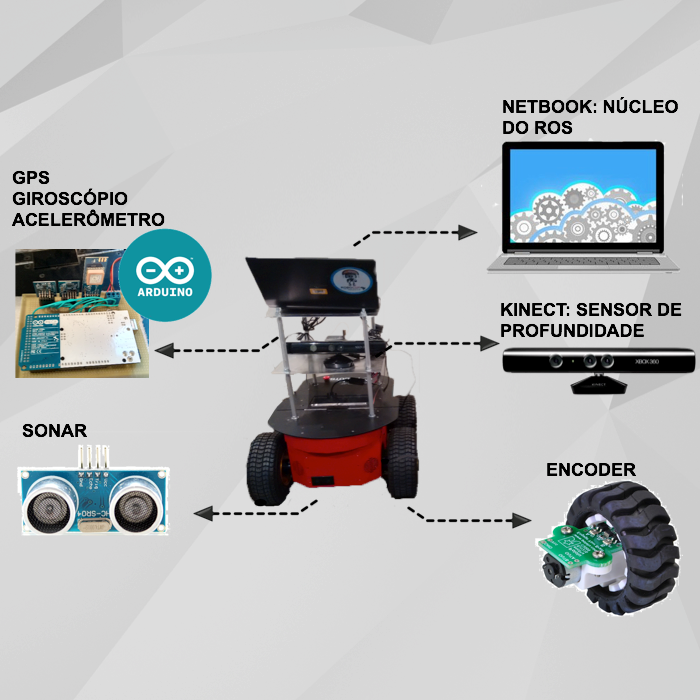
\includegraphics[width=8cm]{images/visaoGeral1.png}
\caption{\small{Visão geral dos sensores do sistema, além do \textit{netbook}.}}
\label{fig:visaoGeral1}
\end{figure} 


Os requisitos funcionais do atual projeto são:
\begin{compactenum}
  \item O robô deve ser teleoperado com um Wiimote, sendo feito o controle de velocidade e direção do robô.
  \item O sistema deve controlar os ângulos vertical e horizontal do Kinect (pan e tilt).
  \item O robô deve navegar autonomamente de forma competente. Considera-se competente uma navegação na qual é possível a detecção de obstáculos baixos e altos, tem-se precisão suficiente para não colidir e é possível um funcionamento prolongado sem necessidade de \textit{reset}.
  \item O sistema deve publicar valores válidos dos sensores (GPS, Acelerômetro e Giroscópio) no ROS.
  \item O sistema deve prover uma visualização tridimensional do ambiente ao redor do robô, enquanto se teleopera o mesmo.
  \end{compactenum}


Os requisitos não funcionais são:
\begin{compactenum}
  \item Uso do \textit{framework} ROS.
  \item Uso do pacote \textit{Navigation Stack} (\verb|move_base| e \verb|gmapping|) para realização do SLAM (\textit{Simultaneous Localization and Mapping}).
  \item Uso do pacote \verb|octomap| para visualização 3D.
  \item Uso das bibliotecas \verb|TinyGPS| e \verb|rosserial| para leitura dos sensor GPS e comunicação entre o microcontrolador e o \textit{master} do ROS.
  \item Uso do microcontrolador Arduino para o controle do servo que gira a base do Kinect, para a leitura dos sensores e para a comunicação com o \textit{master} do ROS.
  \item Uso da biblioteca \verb|wiimote| para comunicação \textit{bluetooth} entre o Wiimote e o ROS.
\end{compactenum}
